\chapter{Deep Generative Models}

A generative model is a statistical model of the data distribution {\bf p}. \\
A discriminative model on the other hand are statistical models of conditional distributions.\\
To generate data there are two general ways: explicit and implicit density estimation. \\
In explicit we find a probability distribution $f \in \triangle{\mathscr{Z}}$ that fits the data, where $z$ is sampled from ${\bf p}_{data}$. \\
In implicit we have to find a function $f$ that generates data $f(\omega) \in \mathscr{Z}$\\
The objective is to find an hypothesis space that can represent probability distributions and that best fits the data.\\
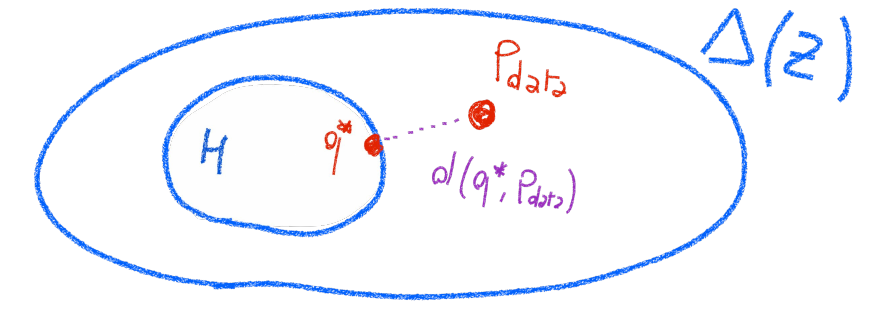
\includegraphics[scale=0.5]{hypothesis}.
\section{Variational Autoencoders (VAE)}
The main idea is to add a probability to traditional autoencoders.\\
Autoencoders are a way of compressing high-dimensional data into a lower dimensional representation (e.g. PCA).\\
An encoder is trained by leveraging a decoder mapping the representation back to the input domain, yielding a reconstruction. \\
This decoder can be used to generate new data although it will not be following the data distribution. \\
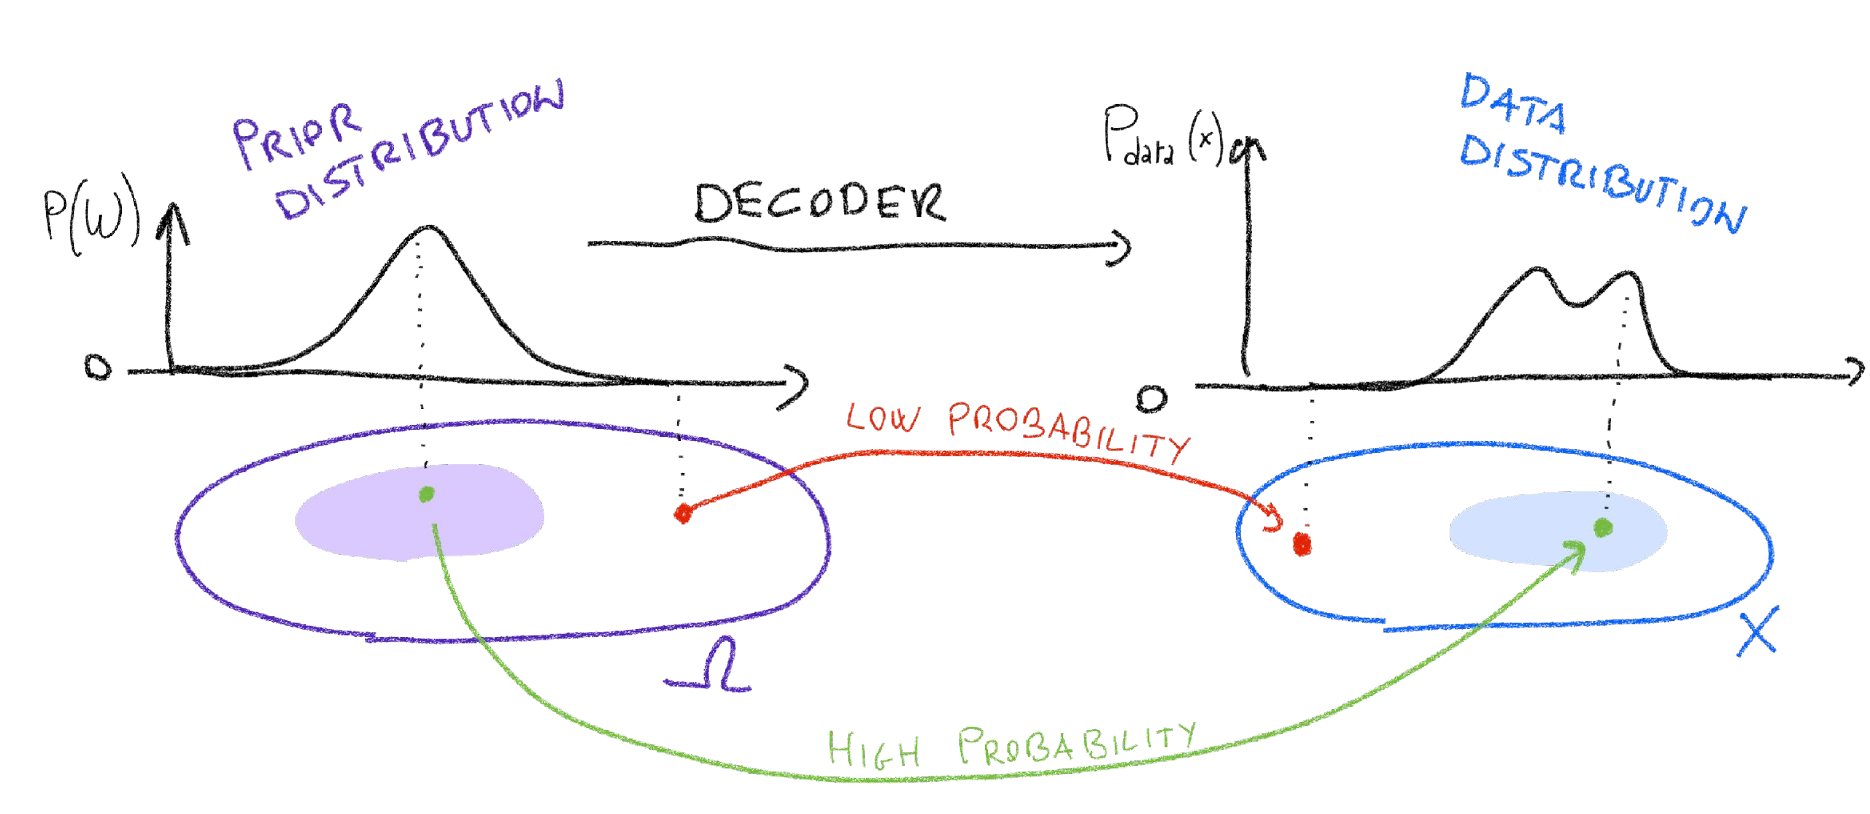
\includegraphics[scale=0.2]{autoencoder}\\
A variation of VAE is the conditional VAE that creates data considering other factors too (generate a person with glasses, for example.)\\
There are of course issues with VAE namely the risk of underfitting and blurry created data. 
\section{Generative Adversarial Networks (GAN)}
GAN enables the possibility of estimating implicit densities. \\
We assume to have already a prior density ${\bf p}_\omega \in \triangle(\Omega)$ and a generator (or decoder) that takes $g\in \mathscr{X}^\Omega$ that generates points in $\mathscr{X}$ given random elements from $\Omega$. \\
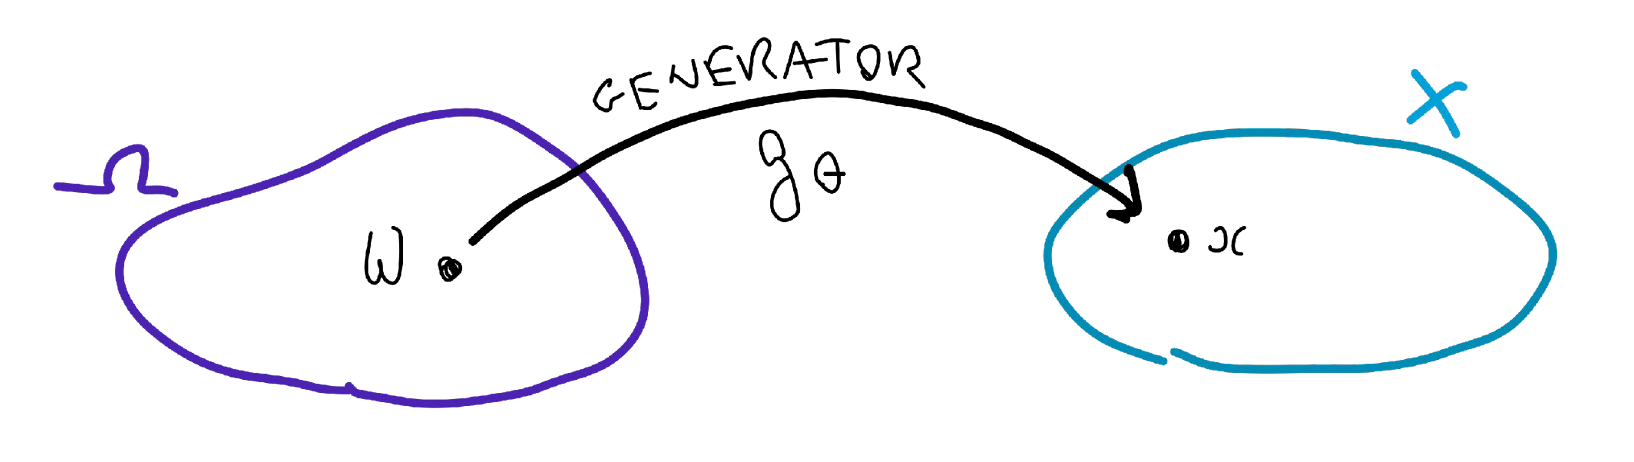
\includegraphics[scale=0.2]{gan} \\
The objective is again to find the best fitting data.\\
The training for GAN works like a one versus one game. Player 1 generates data and player 2 needs to discern whether that's from the original p data or from the newly generated one. This is done with gradient descent \\
Issues are that parameters might not converge and that there might be a vanishing gradient. 